\documentclass[10pt]{article}

\usepackage{ifpdf}
\usepackage{ifxetex}
\usepackage{color}
\usepackage{amsmath}
\usepackage{amsfonts}
\usepackage{booktabs}
\usepackage{tabularx}
\usepackage{colortbl}
\usepackage{multirow}
\usepackage{xcolor}
\usepackage{subfigure}
\usepackage{dcolumn}
\usepackage{flushend}
\usepackage{capt-of}
\usepackage{booktabs}
\usepackage{rotating}
\usepackage{textcomp}

\usepackage{graphicx}
\DeclareGraphicsExtensions{.pdf,.eps,.png,.jpg}
\graphicspath{{./figures/}}

\usepackage{url}

% for border on Verbatim environment
\usepackage{fancyvrb}

% for code listings
\usepackage{listings}

% correct bad hyphenation here
\hyphenation{op-tical net-works semi-conduc-tor}

\newcommand{\DATE}{\today} \newcommand{\LTYPE}{latex2e}
\newcommand{\reffig}[1]{Fig.~\ref{fig:#1}}
\newcommand{\reftab}[1]{Table~\ref{tab:#1}}
\newcommand{\refsec}[1]{Section~\ref{sec:#1}}
\newcommand{\refchap}[1]{Chapter~\ref{chap:#1}}
\newcommand{\reflem}[1]{Lemma~\ref{lem:#1}}
\newcommand{\refthm}[1]{Theorem~\ref{thm:#1}}
\newcommand{\refeq}[1]{Equation~(\ref{eq:#1})}
\newcommand{\ceil}[1]{\left\lceil #1 \right\rceil}
\newcommand{\floor}[1]{\lfloor #1 \rfloor}

\definecolor{Navy}{rgb}{0.1,0.1,0.41}
\definecolor{linkcol}   {named}{Navy}
\definecolor{citecol}   {rgb}{.5,0,0}
\definecolor{urlcol}    {rgb}{0,0,1}

\newcommand{\gprof}{\emph{gprof}}
\newcommand{\DWARV}{\emph{DWARV}}
\newcommand{\TIMES}{$\times$}
\newcommand{\MCPROF}{\emph{MCProf}}

%-----------------------------------------------------------------------------------------
\begin{document}

\title{\MCPROF{}: Memory and Communication Profiler}
\author{Imran Ashraf \\
    Computer Engineering Lab, TU Delft, The Netherlands\\
    I.Ashraf@tudelft.nl
}
\maketitle

%----------------------------------------------------------------------------------
\section{Introduction}
\label{sec:introduction}

\MCPROF{} is a memory and communication profiler. It traces memory reads/writes
and reports memory accesses by various functions in the application as well as
the data-communication between functions. The information is obtained by
performing dynamic binary instrumentation by utilizing Intel Pin \cite{Pin,
Pin_Download} framework.  This manual explains the process of setting up
\MCPROF{} and using it.


%----------------------------------------------------------------------------------
\section{Licensing}

{
\scriptsize
\begin{Verbatim}[frame=single, samepage=true]
Copyright (c) 2014-2015 TU Delft, The Netherlands.
All rights reserved.

MCProf is free software: you can redistribute it and/or modify it under the
terms of the GNU Lesser General Public License as published by the Free
Software Foundation, either version 3 of the License, or (at your option)
any later version.

MCProf is distributed in the hope that it will be useful, but WITHOUT ANY
WARRANTY; without even the implied warranty of MERCHANTABILITY or FITNESS FOR
A PARTICULAR PURPOSE.  See the GNU Lesser General Public License for more details.

You should have received a copy of the GNU Lesser General Public License along
with MCProf.  If not, see <http://www.gnu.org/licenses/>.
\end{Verbatim}
}


%----------------------------------------------------------------------------------
\section{Reference \MCPROF{}}

\subsection{To cite MCProf}

{
\tiny
\begin{Verbatim}[frame=single, samepage=true]
@inproceedings{mcprof,
author = "I. Ashraf and V.M. Sima and K.L.M. Bertels",
title = "Intra-Application Data-Communication Characterization",
booktitle = "Proc. 1st International Workshop on Communication Architectures at Extreme Scale",
address = "Frankfurt, Germany",
month = "July",
year = "2015",
}
\end{Verbatim}
}

% \subsection{To cite MCProf Tool}
% 
% {
% \scriptsize
% \begin{Verbatim}[frame=single, samepage=true]
% "MCProf: Open-source Memory and Communication Profiler"
% Imran Ashraf
% URL: https://bitbucket.org/imranashraf/mcprof
% \end{Verbatim}
% }


%----------------------------------------------------------------------------------
\section{Supported Patforms}
\label{sec:platform}

\MCPROF{} relies on Intel Pin, so it can be used on any 64-bit Linux platform for 
which Pin is available. We have used \MCPROF{} on 64-bit Ubuntu 12.04, Ubuntu 
14.04 on real machines as well as virtual machines running in virtualbox.

%----------------------------------------------------------------------------------
\section{Availability}
\label{sec:availability}

\MCPROF{} can be downloaded from \cite{mcprofDownload}.

To get the latest version, you can clone \MCPROF{} from the git repository by:

{
\small
\begin{Verbatim}[frame=single, samepage=true]
git clone https://imranashraf@bitbucket.org/imranashraf/mcprof.git
\end{Verbatim}
}

In this way, you dont need to download \MCPROF{} each time a new version is released.
You can update your \MCPROF{} by going inside the directory where you have cloned \MCPROF{}
and executing the following commands:

{
\small
\begin{Verbatim}[frame=single, samepage=true]
make clean
git fetch
git pull origin master
\end{Verbatim}
}


%----------------------------------------------------------------------------------
\section{Required Packages}
\label{sec:reqPackages}

In order to setup and use \MCPROF{} the following two packages are required:

\begin{itemize}

\item Intel Pin DBI framework \cite{Pin_Download} Revision 62732 or higher

\item g++ compiler with support for C++11X

\item libelf-dev

\item libdwarf-dev

\item graphviz Dot utility for converting the generated communication graphs
    from DOT to pdf formats

\item gnuplot to plot communication matrix as graph

\end{itemize}

Intel Pin does not need installation. You just need to download the archieve and 
extract to some location. For the remaining packages, you can search on internet 
how to install these packeges in your linux distribution. In Ubuntu 14.04, these 
packages can be installed, for example, by the following commands:

{
\small
\begin{Verbatim}[frame=single, samepage=true]
sudo apt-get install g++
sudo apt-get install libelf-dev
sudo apt-get install libdwarf-dev
sudo apt-get install graphviz
sudo apt-get install gnuplot
\end{Verbatim}
}



%----------------------------------------------------------------------------------
\section{Installation}
\label{sec:installation}

\MCPROF{} uses Makefile to compile the sources. In order to compile \MCPROF{}
from sources on 32-bit / 64-bit Linux, the following steps can be performed.

\begin{itemize}

\item Download Pin and copy and extract it to the directory where you want to
    keep Pin.

\item Define a variable \verb|PIN_ROOT| by running the following commands:

{
\small
\begin{Verbatim}[frame=single]
export PIN_ROOT=/<absolute path to pin directory>
\end{Verbatim}
}

\item Add Pin to your path by the following command:
{
\small
\begin{Verbatim}[frame=single]
export PATH=$PIN_ROOT:$PATH
\end{Verbatim}
}

\item You can also add these lines, for instance, to your \textbf{.bashrc} in case
    you are using \textbf{bash} to export these variables automatically on opening
    a terminal.

\item Download \MCPROF{} and copy and extract it to the directory where you want
    to compile it.

\item Go the \MCPROF{} directory and run the following command to compile it:

{
\small
\begin{Verbatim}[frame=single]
make
\end{Verbatim}
}

\end{itemize}

If every thing goes fine, you will see a directory \verb|obj-intel64| (or
\verb|obj-ia32| depending upon your architecture). This directory will contain
the executables and object files generated as a result of the compilation. The
important files are:

\begin{itemize}

\item \textbf{mcprof.so} which is the tool. This will be used to profile the
    applications as explained in Section \ref{sec:usage}.

\item executable files of the test applications available in \textbf{tests}
    directory.  These executables can be used as test inputs.

\end{itemize}



%----------------------------------------------------------------------------------
\section{Usage}
\label{sec:usage}

In order to explain the usage of \MCPROF{} we will use the example application
listed in Figure \ref{fig:vectOps}. The complete source-code is available in
\textbf{tests} directory of source package. In this application, $4$ \verb|int|
arrays are created on source lines 23, 24, 25 and 26. These arrays are
initialized in \verb|initVecs| function. The sum and difference of the elements
of these arrays are computed in \verb|sumVecs| and \verb|diffVecs| functions,
respectively.  Finally, these arrays are free on lines 32-35.

\begin{figure} %[ht]
    \centering
%     \lstinputlisting[basicstyle=\scriptsize,language=C,showstringspaces=false,frame=bt]{code/example.c}
    \lstinputlisting
    [
    language=C,
    showstringspaces=false,
    frame=bt,
    numbers=left,
    stepnumber=1,
    basicstyle=\small %\tiny
    ] {code/vectOps.c}
    \caption{Example of an application processing some arrays.}
    \label{fig:vectOps}
\end{figure}


\subsection{Profiling Given Tests}

This example will be compiled during the default compilation of the \MCPROF{}
discussed in Section \ref{sec:installation}. In order to profile this
application by \MCPROF{} you can give the following command:

{
\small
\begin{Verbatim}[frame=single]
make vectOps.test
\end{Verbatim}
}

Similarly, other tests can also be executed by replacing the
\textbf{\textlangle vectOps \textrangle.test} with the
\textbf{\textlangle test application name \textrangle.test} as
given in \textbf{tests} directory. This will generate the output information
depending upon the selected engine. The details of the generated output are
provided in Section \ref{sec:output}.

\subsection{Profiling Your Own Example}

In order to provide an example of how you can compile and profile your own
application, the same \textbf{vectOps} example is provided in directory
\textbf{yourApp}. You can copy this directory to any location you like your
Linux machine. In order to profile this application, a \textbf{makefile} is
provided in this directory containing all the rules to compile and profile this
application. You need to make some changes before profiling this application.

\begin{itemize}
\item Modify the path to Pin directory on line 1 in the makefile.
\item Modify the path to \MCPROF{} directory on line 2 in the makefile.
\end{itemize}

In order to avoid these changes in each makefile, you can also add these paths
in \verb|.bashrc| file as:

{
\small
\begin{Verbatim}[frame=single]
export PIN_ROOT=/<absolute path to pin directory>
export PATH=$PIN_ROOT:$PATH
export MCPROF_ROOT=/<absolute path to mcprof directory>
\end{Verbatim}
}

It should be noted that the \MCPROF{} options are provided in \verb|MCPROF_OPT|
variable in \textbf{makefile}. You can modify these options as required. The
details of these options are available in Section \ref{sec:inputopt}. Once these
modifications are performed, this application can be compiled by:

{
\small
\begin{Verbatim}[frame=single]
make mcprof.compile
\end{Verbatim}
}

The above command will generate the binary of the application. Next, to profile
the application by \MCPROF{}, run the following command:

{
\small
\begin{Verbatim}[frame=single]
make mcprof.execute
\end{Verbatim}
}


%----------------------------------------------------------------------------------
\section{\MCPROF{} Input Options}
\label{sec:inputopt}

The complete list of the input options to \MCPROF{} can be obtained by running
the following command:

{
\small
\begin{Verbatim}[frame=single]
pin -t <Path to MCProf dir>/obj-intel64/mcprof.so -h -- ls
\end{Verbatim}
}

Some of the important input options are detailed here.

\begin{description}

\item [-RecordStack] [0/1, default 0] to tell \MCPROF{} to include stack accesses or not.

\item [-TrackObjects] [0/1, default 0] to tell \MCPROF{} if you want to track 
objects. If set 1, the calls to memory allocations functions (malloc, calloc, 
realloc, free, new, delete) will be instrumented to track the allocation and 
deallocation of objects at run-time in the application. The complete call-path 
to the allocation site, with source file-name and line-no information will be 
recorded as well and availble in symbol.out file.

\item [-Engine] [1/2/3, default 2] This selects the engine to be used in
    \MCPROF{}.  Based on the selected engine, the desired output is generated as
    below:

    \begin{description}

    \item [Engine 1]    provides the compute and memory intensive functions and
        objects (if TrackObjects is 1) in the application.

    \item [Engine 2]    provides the data-communication information between
        functions. If TrackObjects is 1, the communication is also reported
        through objects in the application.

    \item [Engine 3]    reports the memory access information through functions
        and objects per call.

    \end{description}

\item [-ShowUnknown]  [0/1, default 0] Show Unknown function in the output graphs.

\item [-TrackStartStop] [0/1, default 0] Track start/stop markers in the code to
    start/stop profiling instead of starting from main().

\item [-TrackZones] [0/1, default 0] Track zone markers to profile per zone. See
    \textbf{markers.c} example available in tests directory. Note \textbf{markers.h}
    include. Also note how this test is compiled and executed in \textbf{makefile.rules}.

\item [-Threshold] [32-bit integer, default 0] to set the threshold value for the 
    output generated by \MCPROF{}. Communication below this threshold will not appear
    in the output graph.

\end{description}

%----------------------------------------------------------------------------------
\section{\MCPROF{} Generated Output}
\label{sec:output}

\MCPROF{} generates various output files based on the selected engines. An
important file which is generated independent of the selected engine is
\textbf{symbols.out}.  This file contains the information about the
function/object symbols tracked during the application execution. In case of
objects, the allocation address, allocation size, call-path of the allocation is
also reported.

\subsection{Engine 1 Output}

The output of Engine 1 are two text-files \textbf{execProfile.out} in the current
directory.

\textbf{execProfile.out} file contains the information about the
execution profile of the application. This profile lists the compute intensive
functions in the application by reporting the percentage of dynamically executed
instructions. An example output for the \textbf{vectOps} application is shown below:

{
\scriptsize
\begin{Verbatim}[frame=single, samepage=true]
%Exec.Instr.        Function Name
==================================
        95          main
        1           diffVecs
        1           sumVecs
        1           initVecs
\end{Verbatim}
}

\textbf{memProfile.out} file contains the information about the memory accesses
performed by functions/objects in the application. An example output for the
\textbf{vectOps} application is shown below:

{
\scriptsize
\begin{Verbatim}[frame=single, samepage=true]
This table can be sorted by Total Accesses (-k2) by using bash command:
    tail -n +7 memProfile.out | sort -k2 -gr

Function   ============ Accesses  ==========    Allocation
 Name       Total         Reads        Writes      Path
===============================================================
UnknownFtn  287038        232876      54162     :0
initVecs    800           0           800       :0
sumVecs     1200          800         400       :0
diffVecs    1200          800         400       :0
main        74982         70976       4006      :0
srcArr1     1200          800         400       /<complete path>/vectOps.c:51
srcArr2     1200          800         400       /<complete path>/vectOps.c:54
sumArr      404           4           400       /<complete path>/vectOps.c:57
diffArr     404           4           400       /<complete path>/vectOps.c:60
\end{Verbatim}
}

The accesses reported against \textbf{UnknownFtn} are the accesses which cannot
be associated to any function. For instance the accesses before starting the
\textbf{main} function is called.

In case of objects, their source-file and line-no information is also reported in
the last column.

\subsection{Engine 2 Output}

\MCPROF{} records data-communication among functions. This is reported as a
data-communication in DOT format in the file \textbf{communication.dot} in the
current directory. This file can be converted to pdf by the following command:

{
\small
\begin{Verbatim}[frame=single]
dot -Tpdf communication.dot -o communication.pdf
\end{Verbatim}
}

A script \verb|dot2pdf.sh| is also provided in the \textbf{scripts} directory which can
also be used to convert the graphs in \emph{dot} format to \emph{pdf} format. This script
also performs some extra tasks, for instance, remove unconnected nodes in the
graph. This script can be used as:

{
\small
\begin{Verbatim}[frame=single]
<path to mcprof dir>/scripts/dot2pdf.sh
\end{Verbatim}
}

Figure \ref{fig:comm} shows the data-communication graph generated by \MCPROF{}
with TrackObjects as 0.

\begin{figure}[!h]
\centering
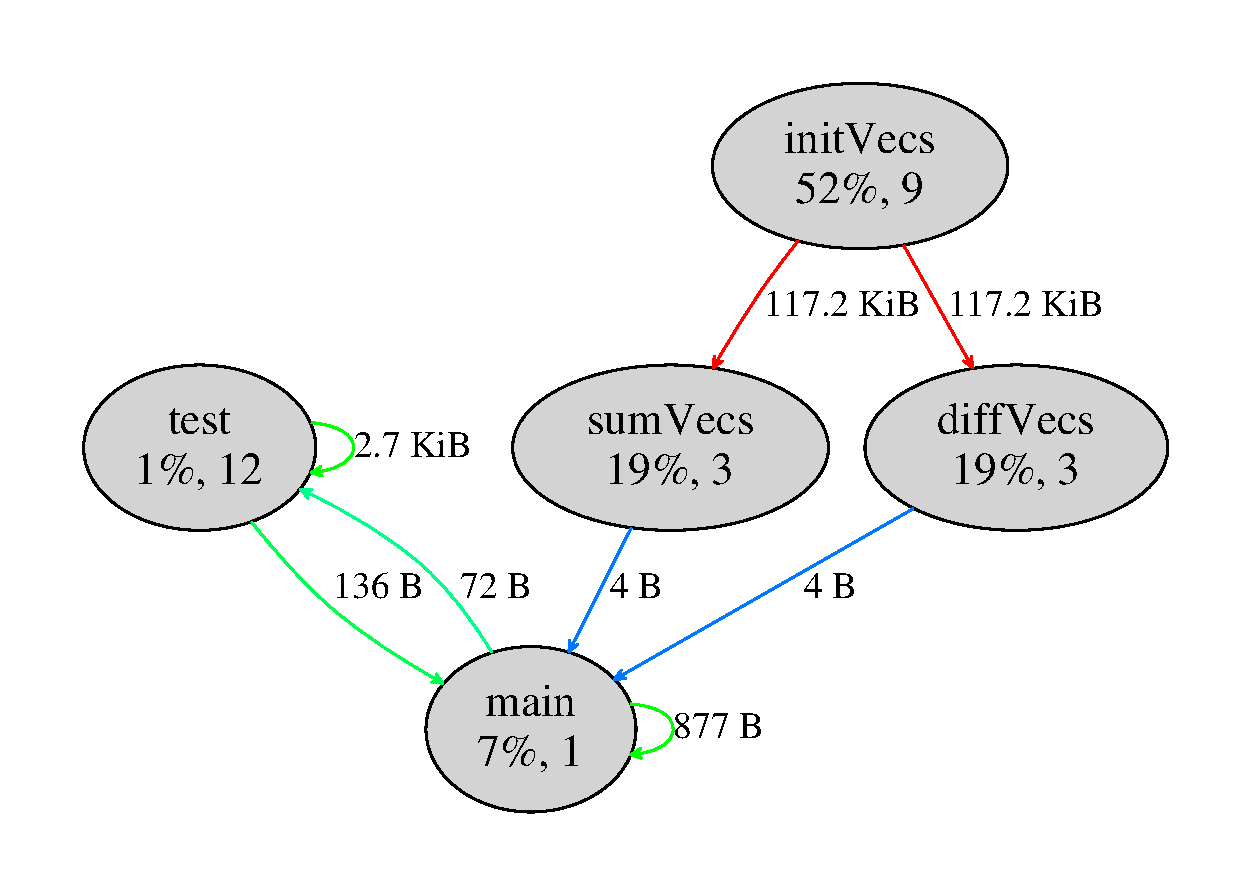
\includegraphics[width=0.55\linewidth]{figures/comm.pdf}
\caption{Data-communication among functions in vectOps application as reported
    by \MCPROF{}. The Grey ovals represent functions. The arcs represent the
    communication with the number on the arc representing the amount of
    data-communication in bytes. The number inside the ovals with \% represent
    the percentage of the dynamically executed instructions. The second number
    is the total calls to this function.}
\label{fig:comm}
\end{figure}

Another important format of the reported information is the data-communication 
matrix. In this format, the communication is reported in the form of a matrix in 
a \textbf{matrix.out} text file. This file can be converted to a graph by using 
\verb|plotScript.sh| script availble in \textbf{scripts} directory. This can be 
executed as:

{
\small
\begin{Verbatim}[frame=single]
<path to mcprof dir>/scripts/plotScript.sh
\end{Verbatim}
}

Figure \ref{fig:matrix} shows the resulting graph for vectOps application.

\begin{figure}[!h]
\centering
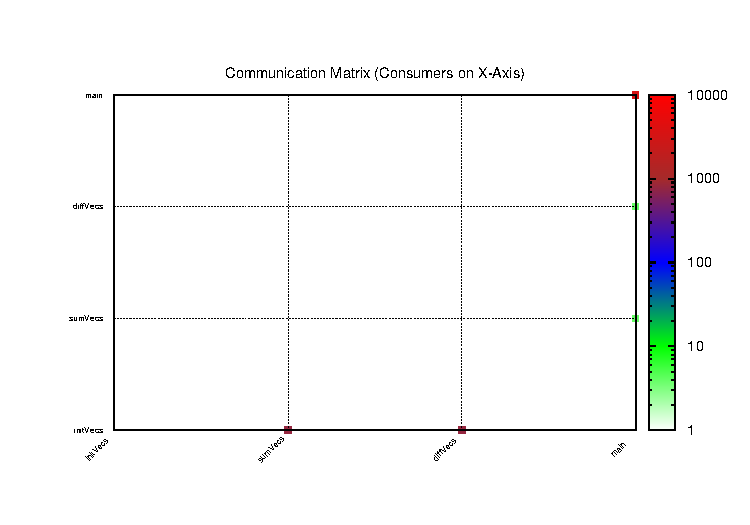
\includegraphics[width=0.95\linewidth]{figures/matrix.pdf}
\caption{Data-communication Matrix showing intensity of communication
    among functions in vectOps application as reported by \MCPROF{}.}
\label{fig:matrix}
\end{figure}


When TrackObjects is set to 1, then the object allocation (malloc/new) are
also tracked and data-communication is reported through these objects. 
Figure \ref{fig:commWithObjects} shows the same graph with TrackObjects as 1.

\begin{figure}[!h]
\centering
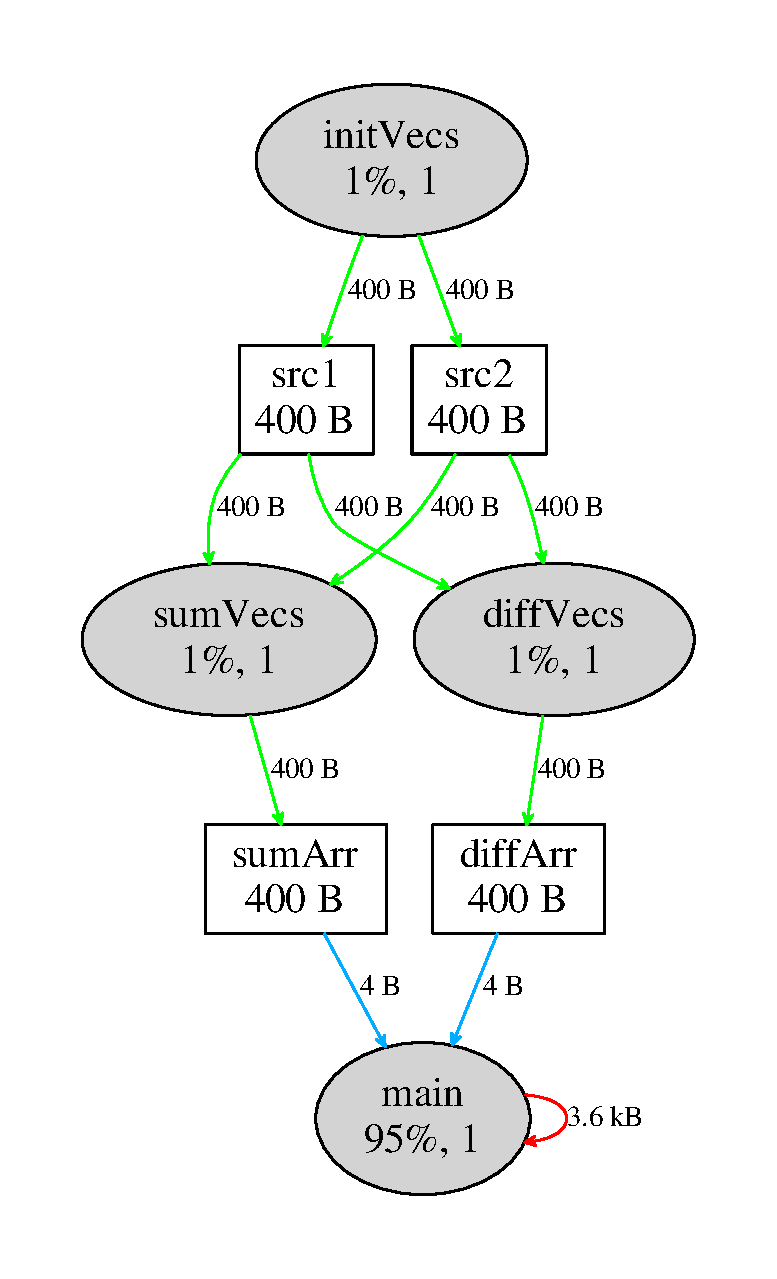
\includegraphics[width=0.55\linewidth]{figures/commWithObjects.pdf}
\caption{Data-communication among functions in vectOps application as reported
    by \MCPROF{}. The tracked objects and communication through these objects
    is also shown. The Grey ovals represent functions. The white rectangles
    represent objects. The number inside the boxes represent the size of this
    object. The arcs represent the communication with the number on
    the arc representing the amount of data-communication in bytes.The number
    inside the ovals with \% represent the percentage of the dynamically
    executed instructions. The second number is the total calls to this function.}
\label{fig:commWithObjects}
\end{figure}

It is important to mention here that the names of the static objects are 
automatically detected by reading (ELF) header (will be available soon). 
However, the names of the dynamic objects are supplied by the user. \MCPROF{} 
provides complete path to the allocation of an object in the source-code. So 
user has to manually look at the source-code to specify what should be the name 
of each object, in order to see the meaningful names of the objects. Hence, the 
user can insert these names directly in \textbf{communication.dot} file. A 
script will also be added soon to automate this process as much as possible.

\subsection{Engine 3 Output}

\MCPROF{} reports per call accesses in Engine 3 in \textbf{percallaccesses.out}
text file, as shown below:

{
\scriptsize
\begin{Verbatim}[frame=single]

Printing All Calls

Printing Calls to initVecs
Total Calls : 1
Call No : 0
Call Seq No : 1
Call Stack : UnknownFtn -> main -> initVecs
Writes to Object5 : 400
Writes to Object6 : 400

Printing Calls to sumVecs
Total Calls : 1
Call No : 0
Call Seq No : 2
Call Stack : UnknownFtn -> main -> sumVecs
Reads from Object5 : 400
Reads from Object6 : 400
Writes to Object7 : 400

Printing Calls to diffVecs
Total Calls : 1
Call No : 0
Call Seq No : 3
Call Stack : UnknownFtn -> main -> diffVecs
Reads from UnknownFtn : 3115
Reads from Object5 : 400
Reads from Object6 : 400
Reads from Object7 : 4
Reads from Object8 : 4
Writes to UnknownFtn : 797
Writes to Object8 : 400

Printing Calls to main
Total Calls : 1
Call No : 0
Call Seq No : 0
Call Stack : UnknownFtn -> main
Reads from UnknownFtn : 69368
Writes to UnknownFtn : 3568
\end{Verbatim}
}


%----------------------------------------------------------------------------------
\section{Frequently Encountered Problems}
\label{sec:faq}

This section will cover some of the frequently encountered problems will
setting-up/using \MCPROF{}.

\subsection{Pin: No such file or directory}
This is because Pin needs 32 bit libraries (See \cite{PinLibs32}).
On Ubuntu, this can be solved by:
{
\small
\begin{Verbatim}[frame=single, samepage=true]
sudo dpkg --add-architecture i386
sudo apt-get update
sudo apt-get install libc6:i386 libncurses5:i386 libstdc++6:i386
\end{Verbatim}
}


\subsection{Pin Injection Mode Error}

On some systems if Pin (parent) injection mode is not enabled by default then
you see an error as shown below.

{
\small
\begin{Verbatim}[frame=single, samepage=true]
E:Attach to pid 13972 failed. 
E:  The Operating System configuration prevents Pin
E:  from using the default (parent) injection mode.
E:  To resolve, either execute the following (as root):
E:  $ echo 0 > /proc/sys/kernel/yama/ptrace_scope
E:  Or use the "-injection child" option.
E:  For more information, regarding child injection,
E:  see Injection section in the Pin User Manual.
\end{Verbatim}
}

Solution is also suggested in this message, which is to become root and enable
this injection. This can be achieved by running the following two commands:

{
\small
\begin{Verbatim}[frame=single, samepage=true]
sudo -i
echo 0 > /proc/sys/kernel/yama/ptrace_scope
exit
\end{Verbatim}
}


%----------------------------------------------------------------------------------
\section{Contact}
\label{sec:contact}

In case you are interested in contributing to \MCPROF{}, or you have suggestions
for improvements, or you want to report a bug, contact:

\begin{itemize}
\item Imran Ashraf \textlangle I.Ashraf@TUDelft.nl \textrangle
\end{itemize}

%----------------------------------------------------------------------------------
% references section
\bibliographystyle{unsrt}
\bibliography{bib/references}

% that's all folks
\end{document}
%----------------------------------------------------------------------------------



% An example of an equation \ref{eq:amdhal}.
% \begin{equation}
% \label{eq:amdhal}
% \lim_{p \to \infty} \frac{p}{1-f(p-1)} = \frac{1}{f} = \frac{1}{1-s},
% \end{equation}
%  where $p$ is the speedup factor of the accelerated part, $f$ is the percentual
% contribution of the sequential part, and $s$ is the original percentual
% contribution of the accelerated part.
